\documentclass[12pt]{article}

%%%%%%%%%%%%PACKAGES%%%%%%%%%%%%%%
\usepackage[top=2cm,bottom=2cm, right = 1cm, left = 1.5cm]{geometry}
\usepackage{fancyhdr}

\usepackage[T2A]{fontenc}
\usepackage[english, russian]{babel}
\usepackage{tempora}% bold titles and nice style
\usepackage{graphicx}%%%allow inserting images
\usepackage{xcolor}
\usepackage{enumitem}
\usepackage{float}
%%%%%%%%%%%%%%%%%%%%%%%%%%%%%%%%%

%%%%%%%%%%%%%%%%%%%%%%%%%%preambules%%%%%%%%%%%%%%%%%%%%
%%%%%%%%%%%%%%%%%%%%%%%%%%%%%%%%%%%%%%%%%%%%%%%%%%%%%%%%

\pagestyle{fancy}
\fancyhead{}
\fancyfoot{}%clear all the footnotes
\fancyhead[L]{\slshape\MakeUppercase{РУДН}}
\fancyhead[R]{\slshape{python}}
\fancyfoot[C]{\thepage}%set the notes as the page number
\setlength{\parskip}{0.5em} %lenght between paragrahs
\renewcommand{\baselinestretch}{1.2}%spacing between lines
\parindent 0ex %remove the espace of the first line in every paragraph

%%%%%%%%%%%%%%%%%%%%%%%%%%custom colors%%%%%%%%%%%%%%%%%%%%%%%%%%
%%%%%%%%%%%%%%%%%%%%%%%%%%%%%%%%%%%%%%%%%%%%%%%%%%%%

\usepackage{listings}
\definecolor{codegreen}{rgb}{0.1,0.7,0.1}
\definecolor{codegray}{rgb}{0.5,0.5,0.5}
\definecolor{codepurple}{rgb}{0.7,0,0.98}
\definecolor{codemagenta}{rgb}{1,0,1}
\definecolor{backcolour}{rgb}{1,1,1}
\definecolor{aqua}{rgb}{0.0, 1.0, 1.0}
\definecolor{myyellow}{rgb}{0.9, 0.9, 0.0}

%%%%%%%%%%%%%%%%%%%%%%%%%listing styles%%%%%%%%%%%%%%%%%%%%%%%%%%
%%%%%%%%%%%%%%%%%%%%%%%%%%%%%%%%%%%%%%%%%%%%%%%%%%%%

\usepackage{listings}

\lstdefinestyle{conlst}{
	morekeywords={[1] .py},
	keywordstyle={ [1]\color{orange} },
	basicstyle=\Large\ttfamily,
	commentstyle=\color{gray} \emph,
	stringstyle=\ttfamily,
	backgroundcolor=\color{backcolour},
	stringstyle=\color{codegreen},
	showspaces=false,
	showtabs=false,
	breaklines=true,
	showstringspaces=false,
	breakatwhitespace=true,
	upquote=true,
	frame=tblr,
	escapechar =@,
	columns=fullflexible
	%aboveskip=20pt,
	%belowskip=20pt
	}

\lstdefinestyle{pylst}{
	language=Python,
	morekeywords={[1] None, True, False},
	morekeywords={[2] __init__, __name__},
	morekeywords={[3] self},
	basicstyle=\Large\ttfamily,
	keywordstyle={[1]\color{blue}},
	keywordstyle={[2]\color{codemagenta}},
	keywordstyle={[3]\color{codepurple}},
	keywordstyle={[4]\color{codegreen}},
	commentstyle=\color{codegreen} \emph,
	%stringstyle=\ttfamily,
	numbers=left,
	numberstyle=\small, 
	stepnumber=1, 
	numbersep=5pt,
	backgroundcolor=\color{backcolour},
	stringstyle=\color{orange},
	showspaces=false,
	showtabs=false,
	breaklines=true,
	showstringspaces=false,
	breakatwhitespace=true,
	upquote=true,
	frame=tblr,
	escapechar =@,
	columns=fullflexible,
	%aboveskip=20pt,
	%belowskip=20pt
	}

\lstset{literate=%
   *{0}{{{\color{codegreen}0}}}1
    {1}{{{\color{codegreen}1}}}1
    {2}{{{\color{codegreen}2}}}1
    {3}{{{\color{codegreen}3}}}1
    {4}{{{\color{codegreen}4}}}1
    {5}{{{\color{codegreen}5}}}1
    {6}{{{\color{codegreen}6}}}1
    {7}{{{\color{codegreen}7}}}1
    {8}{{{\color{codegreen}8}}}1
    {9}{{{\color{codegreen}9}}}1
}

%%%%%%%%%%%%%%%%%%%%%%%%%%%%%%%%%%%%%%%%%%%%%%%%%%%%%%%%%%
%%%%%%%%%%%%%%%%%%%%%%%%%%%%%%%%%%%%%%%%%%%%%%%%%%%%%%%%%%
\begin{document}
\tableofcontents
\newpage
\setcounter{page}{1}%set this page as the first page
\section{Требования}
\begin{enumerate}
	\item подключение к интернету
  \item интернет браузер
\end{enumerate}
\section{получить путь к проекту django}
    \subsection{ войти в папку виртуальной среды}
			\begin{lstlisting}[caption=\phantom{},style=conlst,label={lst:enter_desktop}]
      cd djangoEnv/
			\end{lstlisting}
	\begin{figure}[H]
		\centering
		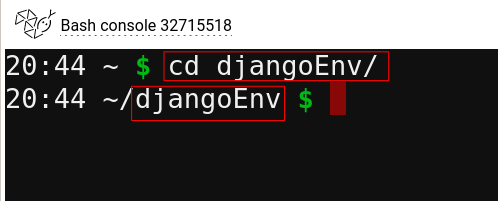
\includegraphics[width=0.4\textwidth ,keepaspectratio]{~/django_project/manuals/imgs/enter_venv_folder.png}
		\caption{}
	\end{figure}
    \subsection{войдите в папку <<websiteRoot>>}
			\begin{lstlisting}[caption=\phantom{},style=conlst,label={lst:enter_desktop}]
      cd websiteRoot
			\end{lstlisting}
	\begin{figure}[H]
		\centering
		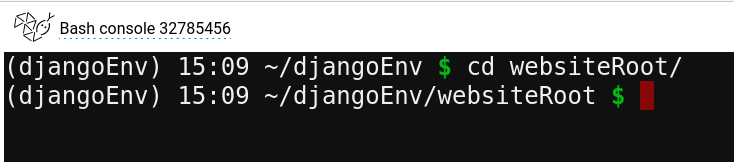
\includegraphics[width=0.3\textwidth ,keepaspectratio]{~/django_project/manuals/imgs/enter_websiteRoot.png}
		\caption{}
	\end{figure}
    \subsection{получить путь к папке <<websiteRoot>>}
			\begin{lstlisting}[caption=\phantom{},style=conlst,label={lst:enter_desktop}]
      pwd
			\end{lstlisting}
	\begin{figure}[H]
		\centering
		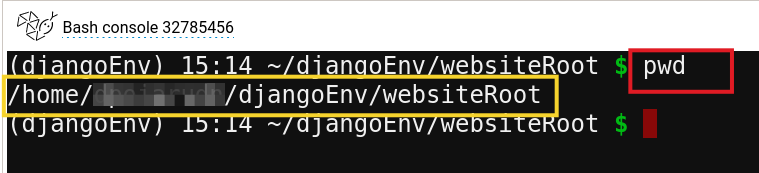
\includegraphics[width=0.3\textwidth ,keepaspectratio]{~/django_project/manuals/imgs/get_websiteRoot_path.png}
		\caption{}
	\end{figure}

    \subsection{выделите путь к папке <<websiteRoot>>, чтобы скопировать его}
	\begin{figure}[H]
		\centering
		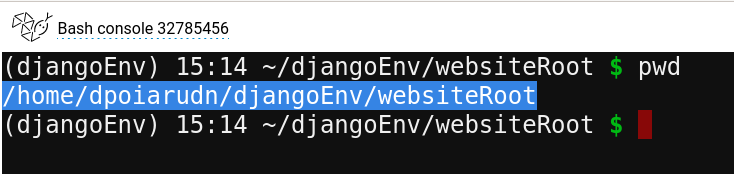
\includegraphics[width=0.4\textwidth ,keepaspectratio]{~/django_project/manuals/imgs/highlight_root_path.png}
		\caption{}
	\end{figure}
  \subsection{вставьте путь, который вы только что скопировали, в текстовый файл, чтобы не потерять его}
	\begin{figure}[H]
		\centering
		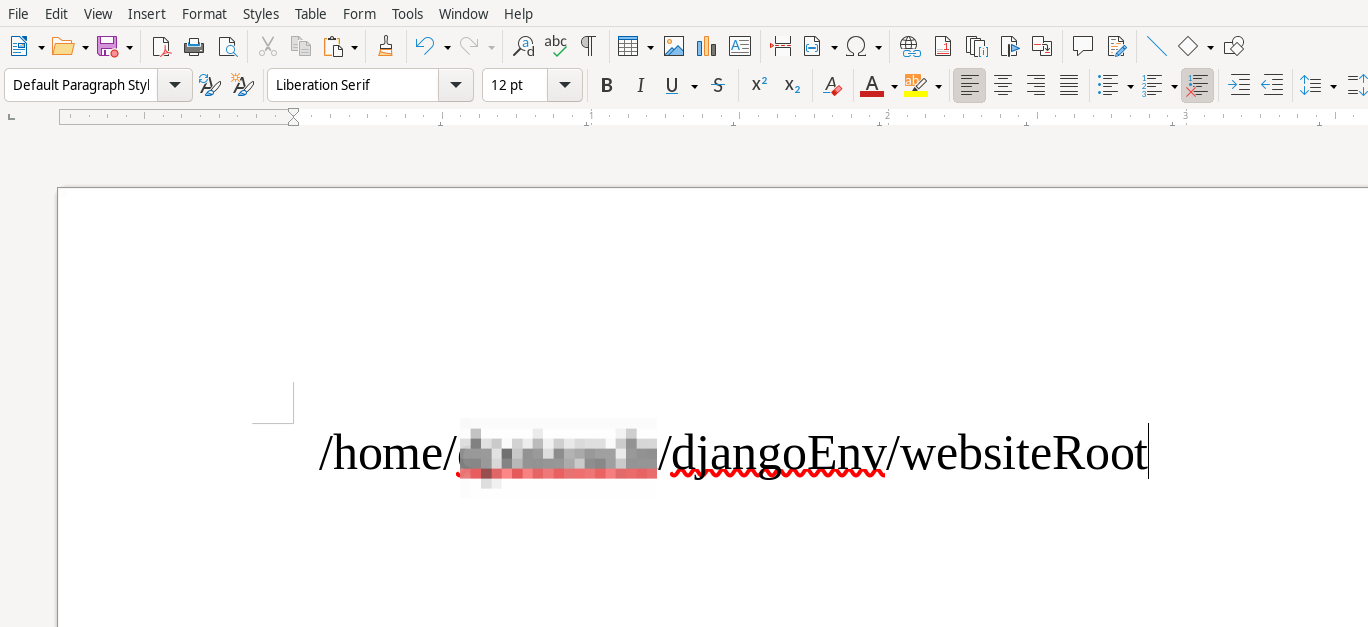
\includegraphics[width=0.4\textwidth ,keepaspectratio]{~/django_project/manuals/imgs/path_libreoffice.png}
		\caption{}
	\end{figure}
    \subsection{ выйти из терминала}
			\begin{lstlisting}[caption=\phantom{},style=conlst,label={lst:enter_desktop}]
      exit
			\end{lstlisting}
	\begin{figure}[H]
		\centering
		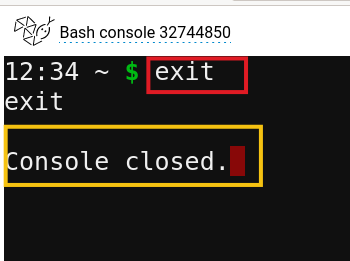
\includegraphics[width=0.3\textwidth ,keepaspectratio]{~/django_project/manuals/imgs/exit_terminal.png}
		\caption{}
	\end{figure}
\section{создать веб-приложение в pythonAnywhere}
    \subsection{ перейдите на следующий веб-сайт и войдите в систему, используя свои учетные данные}
      \begin{lstlisting}[caption=\phantom{},style=conlst,label={lst:enter_desktop}]
      https://www.pythonanywhere.com/
			\end{lstlisting}
    \subsection{нажмите на <<open web tab>>}
	\begin{figure}[H]
		\centering
		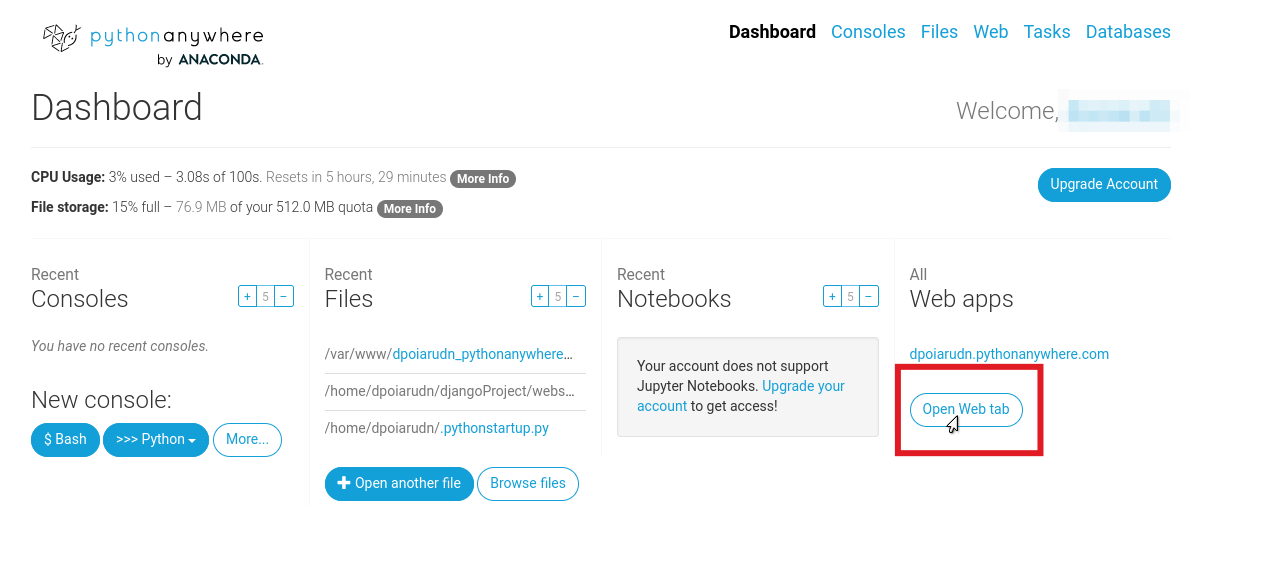
\includegraphics[width=0.3\textwidth ,keepaspectratio]{~/django_project/manuals/imgs/open_web_tab.png}
		\caption{}
	\end{figure}
    \subsection{нажмите на <<add new web app>> и потом нажмите <<next>>}
	\begin{figure}[H]
		\centering
		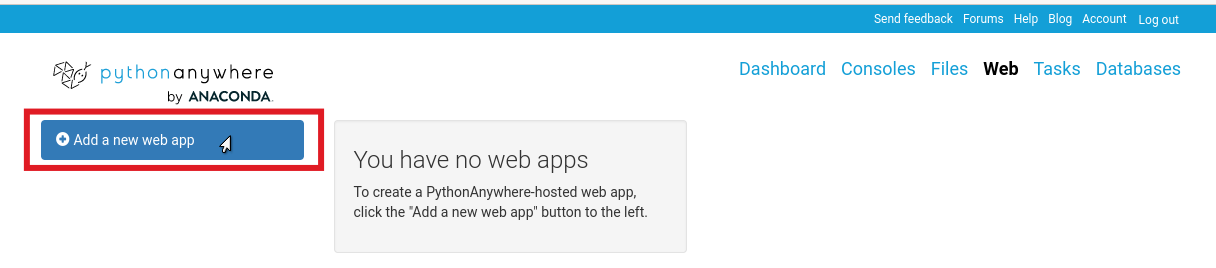
\includegraphics[width=0.3\textwidth ,keepaspectratio]{~/django_project/manuals/imgs/add_web_app.png}
		\caption{}
	\end{figure}
	\begin{figure}[H]
		\centering
		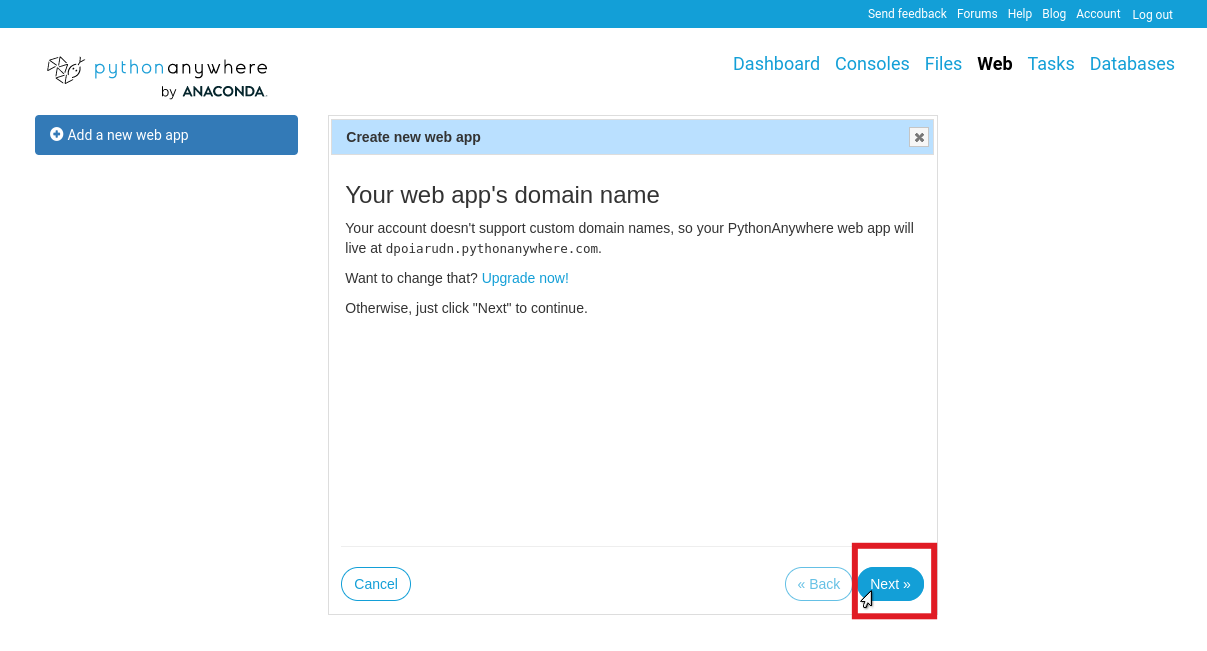
\includegraphics[width=0.3\textwidth ,keepaspectratio]{~/django_project/manuals/imgs/webapp_domain_name.png}
		\caption{}
	\end{figure}
  \subsection{выберите платформу веб-приложения как <<manual configuration>>}
	\begin{figure}[H]
		\centering
		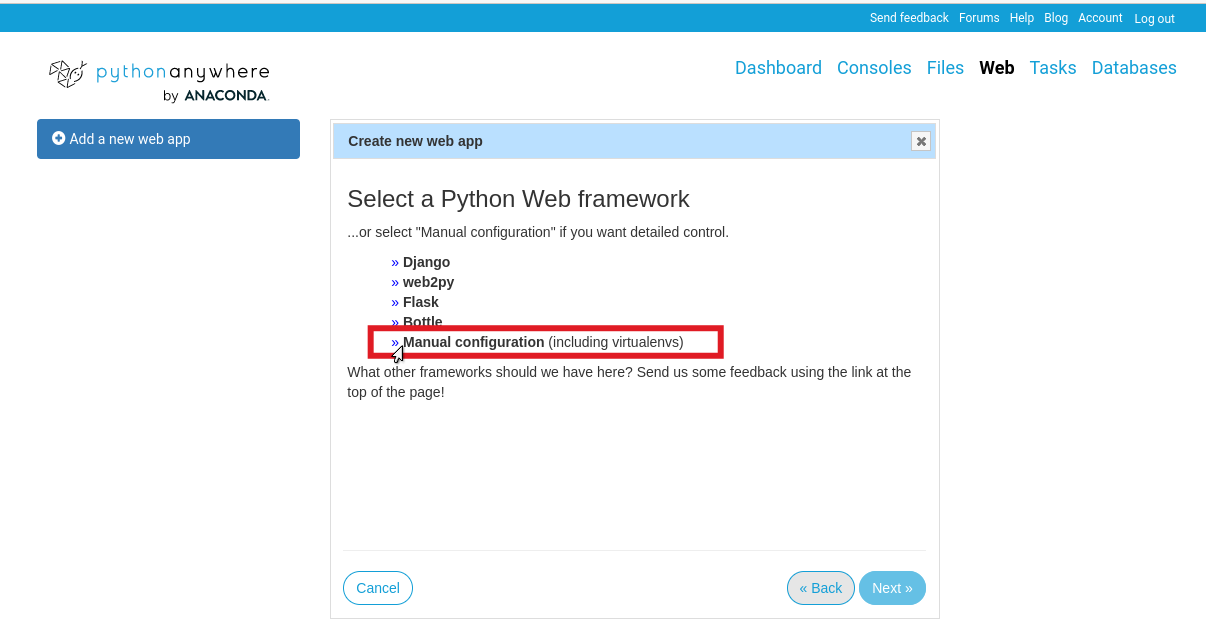
\includegraphics[width=0.3\textwidth ,keepaspectratio]{~/django_project/manuals/imgs/webapp_framework_selection.png}
		\caption{}
	\end{figure}
  \subsection{выберите версию python для использования в веб-приложении (должна соответствовать версии python виртуальной среды). выберите python 3.10 и потом нажмите <<next>>}
	\begin{figure}[H]
		\centering
		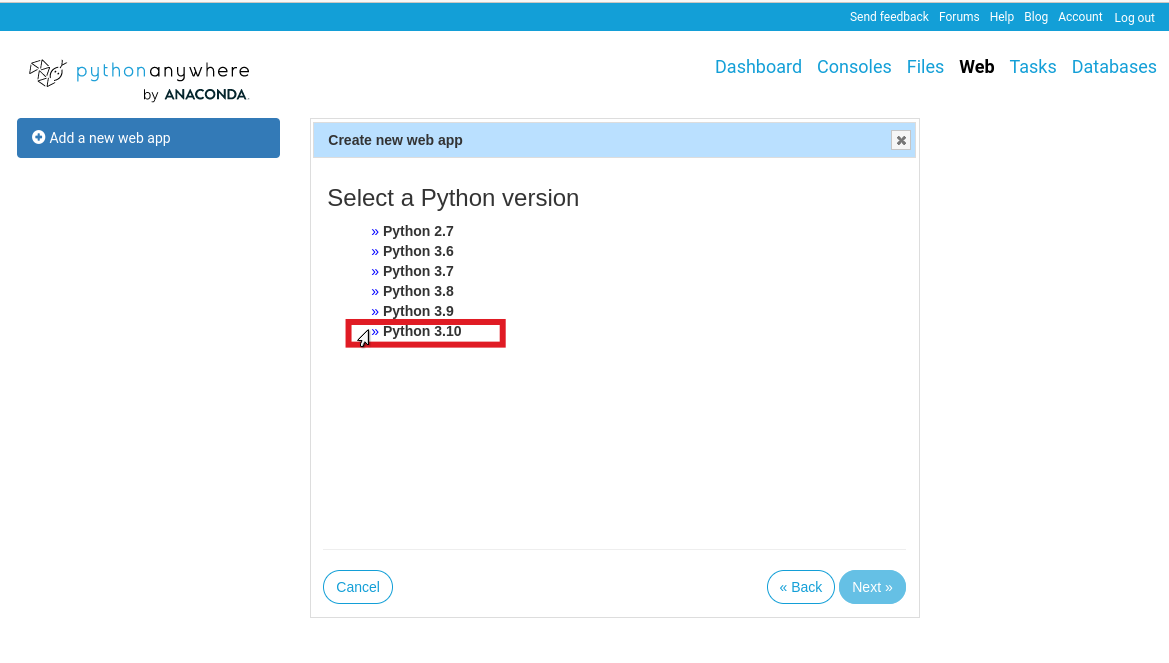
\includegraphics[width=0.3\textwidth ,keepaspectratio]{~/django_project/manuals/imgs/webapp_python_version_selection.png}
		\caption{}
	\end{figure}
	\begin{figure}[H]
		\centering
		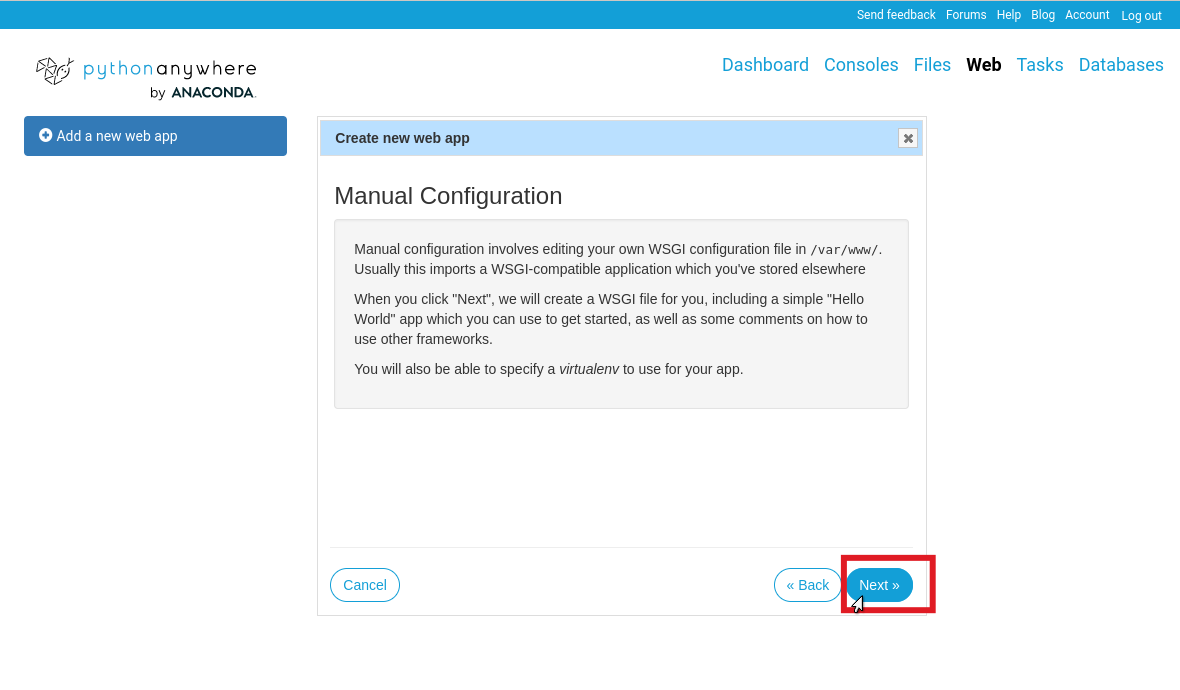
\includegraphics[width=0.3\textwidth ,keepaspectratio]{~/django_project/manuals/imgs/manual_config_next.png}
		\caption{}
	\end{figure}
  \subsection{проверьте, появляется следующая страница}
	\begin{figure}[H]
		\centering
		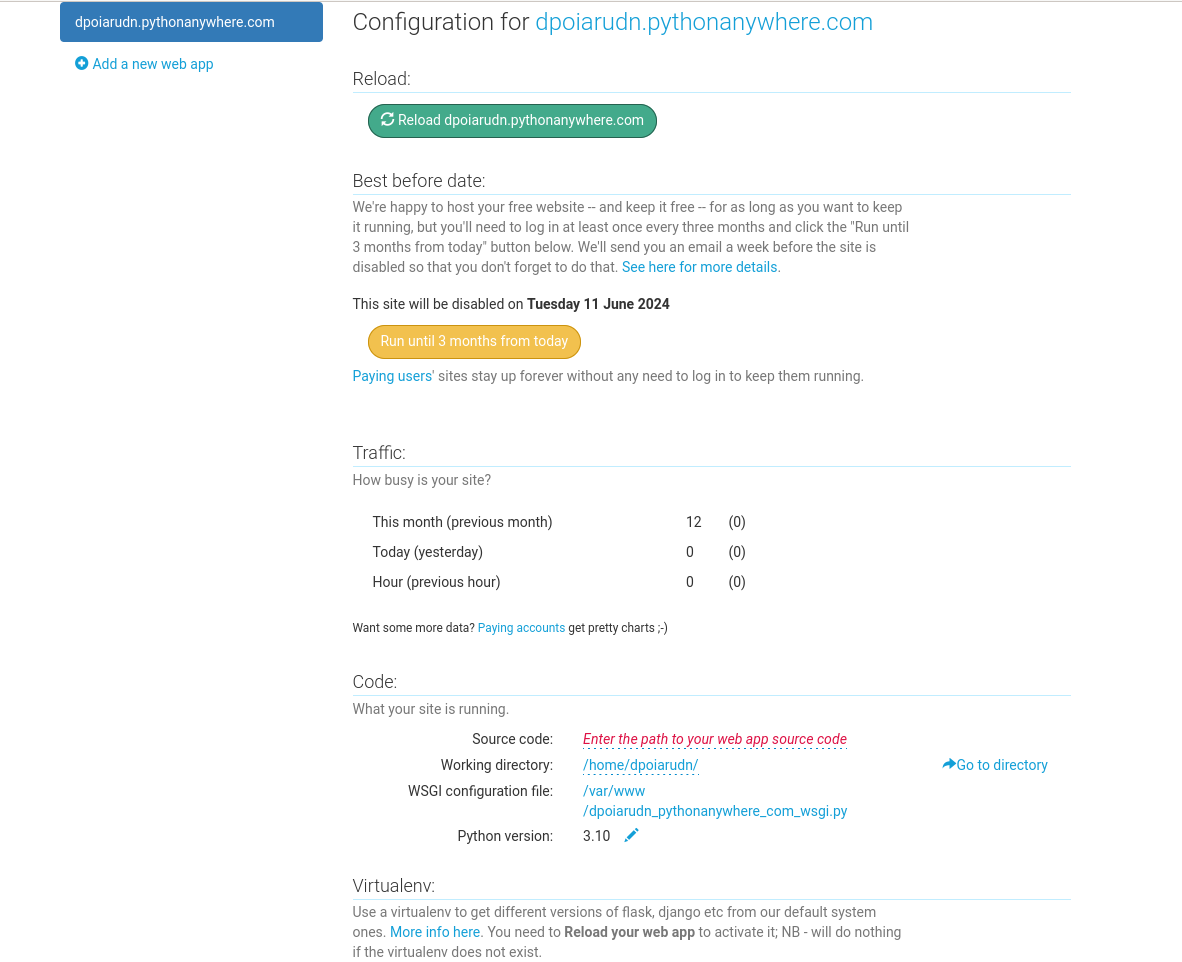
\includegraphics[width=0.3\textwidth ,keepaspectratio]{~/django_project/manuals/imgs/webapp_config_page.png}
		\caption{}
	\end{figure}
  \section{настроить веб-приложение в pythonAnywhere}
  \subsection{зайти в раздел <<virtualEnv>> и вставьте путь, который вы скопировали перед удалением <<websiteRoot>> с пути. и нажмите на галочку.}
	\begin{figure}[H]
		\centering
		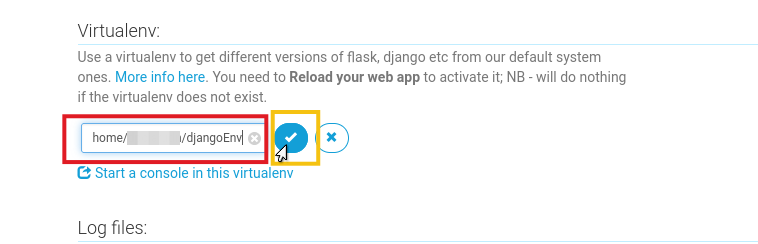
\includegraphics[width=0.3\textwidth ,keepaspectratio]{~/django_project/manuals/imgs/virtual_env_path.png}
		\caption{}
	\end{figure}
	\begin{figure}[H]
		\centering
		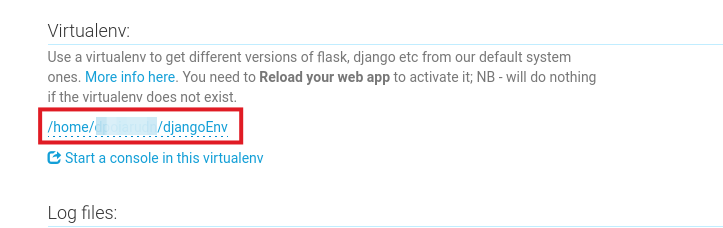
\includegraphics[width=0.3\textwidth ,keepaspectratio]{~/django_project/manuals/imgs/virtual_env_path2.png}
		\caption{}
	\end{figure}
  /home/dpoiarudn/djangoEnv/websiteRoot
\end{document}
